%
%  kant.five
%
%  Created by Mark Eli Kalderon on 2007-08-05.
%  Copyright (c) 2007 Mark Eli Kalderon. All rights reserved.
%
%  Beamer

% Definitions and macros
\newcommand{\change}{\textcolor{blue}{\textbf{CHANGE SLIDE}}}
\def\myauthor{Mark Eli Kalderon} 
\def\mytitle{Introduction to Moral Philosophy}
\def\mysubtitle{Kant}
\def\myinstitution{University College London}
\def\myurl{http://markelikalderon.com/teaching/}

% Packages specific to lecture notes
\mode<article>{
    \usepackage{palatino}
}

% Packages specific to beamer presentation
\mode<presentation>{
    \usetheme{Darmstadt}
    \setbeamercovered{transparent}
    \pgfdeclareimage[height=0.5cm]{university-logo}{../../graphics/logo_sml_blk}
    \logo{\pgfuseimage{university-logo}}
}

% Packages common to lecture notes and beamer presentation
\usepackage{pgf}
\usepackage{tikz}
\usepackage{hyperref}

\setjobnamebeamerversion{kant.five.beamer}

\title{\mytitle}
\subtitle{\mysubtitle} % (optional)

\author{\myauthor\\
\url{\myurl}}
\institute{\myinstitution}

% \date[Short Occasion] % (optional)
% {Date / Occasion}

\begin{document}

\frame{\maketitle}

\section{The Third Formula}

\change\ Kant's search for the supreme principle of morality began with the concept of a categorical imperative which yielded the first formula. The first formula represents the \emph{form} of the moral law, its validity for all rational beings. Kant then considered the motive for following a categorical imperative which yielded the second formula (the Formula of Humanity). The second formula represents the \emph{matter} of the moral law, the end involved in acting from a law valid for all rational beings. From these:

\begin{quote}
there follows now the third practical principle of the will, as supreme condition of its harmony with universal practical reason, the idea of the will of every rational being as a will giving universal law. (G 4:431)
\end{quote}

The third formula has two variants:
\begin{enumerate}
    \item \textbf{The Formula of Autonomy}: ``\ldots the idea of the will of every rational being as a will giving universal law''. (G 4:431; 4:432)
    \item \textbf{The Formula of the Kingdom of Ends}: ``Act in accordance with the maxims of a member giving universal laws for a merely possible kingdom of ends''. (G 4:439; 4:433; 4:437; 4:438)
\end{enumerate}

\change

\begin{frame}<presentation>[label=slide1]
    \frametitle{The Third Formula}
        \begin{columns}
            \begin{column}{3cm}
                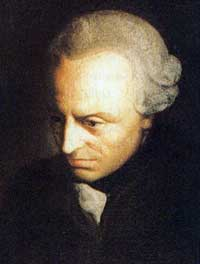
\includegraphics[height=4cm]{../../graphics/kant.jpg}
            \end{column}
            \begin{column}{7cm}
                \begin{enumerate}
                    \item \textbf{The Formula of Autonomy}: ``\ldots the idea of the will of every rational being as a will giving universal law''. (G 4:431; 4:432)
                    \item \textbf{The Formula of the Kingdom of Ends}: ``Act in accordance with the maxims of a member giving universal laws for a merely possible kingdom of ends''. (G 4:439; 4:433; 4:437; 4:438)
                \end{enumerate}
            \end{column}
        \end{columns}
\end{frame}

\section{Autonomy}

The Formula of Autonomy is not formulated as an imperative, at least not initially, but it is easy to see how it might be. In the \emph{Lectures on Ethics} Kant puts it this way: ``So act that by the maxim of your action you present yourself as a will giving universal law'' (27:518). This is very similar to the Formula of Universal Law, but there is a crucial difference. The Formula of Universal Law focuses on our obeying laws valid for all rational beings, the Formula of Autonomy focuses one our being potential \emph{authors} of laws valid for all rational beings. Indeed it is our status as potential authors of universal law that is the ground of our dignity.

Consider two ways in which a person might obey a law.

First, a person might obey a law in order to avoid the sanctions imposed by some external authority (the state or God, say). If a person obeys the law merely to avoid these sanctions, then he is subject to the law. The person's reason for obedience would be to avoid externally imposed sanctions that he fears. If these sanctions ceased to be enforced, or if he ceased to fear them, then the person would no longer have a reason to obey the law.

A person might obey the law by being subject to it, but this is not the only way to obey a law. A person might obey the law, not because of any external incentive, but because he is the author of it. In legislating a law, a person is bound to it, not by any external incentive, but by the reasons he recognized in legislating it. Even if no sanctions were enforced, the person, as the author of the law, would still have a reason to obey the law.

Kant's idea is that our motivation to obey the moral law could not be grounded in external incentive. External incentive depends on inclination which can vary from one rational being to another. So if we were merely subject to the moral law, it would not be valid for every rational being. The motive for obeying the law must be grounded in our status as potential authors of universal law. In legislating a universal law, a person would be bound to it, not by external incentive, but by the reasons he would recongize in legislating it. So even in the absence of external incentive, a person, as the potential author of the moral law, would still have a reason to obey the law.

It is our humanity, our capacity to set ends for reasons, that makes us potential authors of universal law. Moreover, it is because our humanity makes us potential authors of universal law that it can be said to have dignity, a value that cannot be measured against a mere price:

\begin{quote}
For, nothing can have a worth other than that which the law determines for it. But the lawgiving itself, which determines all worth, must for this very reason have a dignity, that is, an unconditional, incomparble worth; and the word repsect alone provides a becoming expression for the estimate of it that a rational being must give. \emph{Autonomy} is therefore the ground of the dignity of human nature and of every rational nature. (G 4:436)
\end{quote}

The Formula of Autonomy makes explicit the value of humanity, its dignity. Moreover, it is this dignity that makes it intelligible that humanity should be the end involved in acting from a moral law valid for every rational being. \change

\begin{frame}<presentation>[label=slide2]
    \frametitle{Autonomy}
        \begin{columns}
            \begin{column}{3cm}
                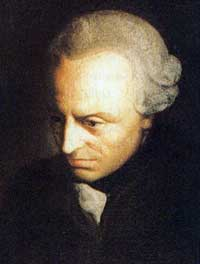
\includegraphics[height=4cm]{../../graphics/kant.jpg}
            \end{column}
            \begin{column}{7cm}
                \begin{itemize}
                    \item \alert{Being subject to a law} versus \alert{being the author of the law}
                    \item Autonomy as the grounds of human dignity
                \end{itemize}
            \end{column}
        \end{columns}
\end{frame}

\section{The Kingdom of Ends}

Like the Formula of Humanity, the Formula of the Kindgom of Ends is strikingly resonant:
\begin{itemize}
    \item \emph{The Formula of the Kingdom of Ends}: ``Act in accordance with the maxims of a member giving universal laws for a merely possible kingdom of ends''. (G 4:439; 4:433; 4:437; 4:438)
\end{itemize}

The Formula of the Kingdom of Ends is a variant of the Formula of Autonomy, and in some places, Kant writes as if it were a mere restatement of it. How are we to understand the connection? Begin with autonomy, ``\ldots the idea of the will of every rational being as a will giving universal law.'' (G 4:431; 4:432). In the Formula of the Kingdom of Ends, Kant claims that these laws would be the laws of a merely possible kingdom of ends. To understand the connection, then, we must understand what Kant means by a ``kingdom of ends''.

Kant defines a \textbf{kingdom} as ``a systematic union of various rational beings through common laws'' (G 4:433). Rational beings constitute a kingdom to the extent that their ends constitute a \textbf{system}. To constitute a system not only must their ends be mutually compatible, but they must be mutually reinforcing as well---they must constitute a system of shared ends. Universal adherence to the laws of a kingdom of ends would result in furthering the ends of all rational beings in a single teleological system. \change

\begin{frame}<presentation>[label=slide3]
    \frametitle{The Kingdom of Ends}
        \begin{columns}
            \begin{column}{3cm}
                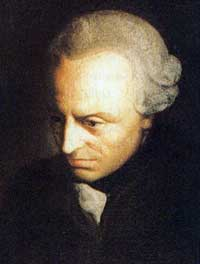
\includegraphics[height=4cm]{../../graphics/kant.jpg}
            \end{column}
            \begin{column}{7cm}
                \begin{itemize}
                    \item \alert{The Formula of the Kingdom of Ends}: ``Act in accordance with the maxims of a member giving universal laws for a merely possible kingdom of ends''. (G 4:439; 4:433; 4:437; 4:438)
                    \item A \alert{kingdom} is ``a systematic union of various rational beings through common laws''. (G 4:433)
                \end{itemize}
            \end{column}
        \end{columns}
\end{frame}

\section{The Derivation}

The derivation of the Formula of the Kingdom of Ends draws on ideas expressed in all previous formulas:

\begin{quote}
For, all rational beings stand under the \emph{law} that each of them is to treat himself and all others \emph{never merely as a means} but always \emph{at the same time as ends in themselves}. But from this there arises a systematic union of rational beings through common objective laws, that is, a kingdom, which can be called a kingdom of ends (admittedly only an ideal) because what these laws have as their purpose is just the relation of these beings to one another as ends and means. (G 4:433)
\end{quote}

Kant begins by combining the idea of acting in conformity with universal law with a characterization of that law as the injunction to treat humanity as an end in itself. Kant then claims that all rational beings stand under ``common objective laws.'' These require that all rational beings be treated as ends in themselves. This requires that we bring our ends into agreement with the ends of the beings so treated. (Recall, especially, Kant's discussion of false promises in terms of the Formula of Humanity.) Legislating common objective law is an action, and all actions have ends, so it is natural for Kant to assume that there is an end involved in legislating common objective law. This must be a single end in which the ends of all rational beings are brought into agreement. There would thereby be a kingdom in which the ends of all rational beings are systematically united in a single share end.

The Formula of the Kingdom of Ends elaborates what was implicit in applying the Formula of Humanity. Specifically, it requires that we exclude ends that could not, in principle, be shared between rational beings (such as those requiring false promises) and that we further ends that unite rational beings (such as rendering mutual aid). \change

\begin{frame}<presentation>[label=slide4]
    \frametitle{The Derivation}
        \begin{columns}
            \begin{column}{3cm}
                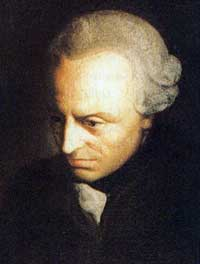
\includegraphics[height=4cm]{../../graphics/kant.jpg}
            \end{column}
            \begin{column}{7cm}
                For, all rational beings stand under the \emph{law} that each of them is to treat himself and all others \emph{never merely as a means} but always \emph{at the same time as ends in themselves}. But from this there arises a systematic union of rational beings through common objective laws, that is, a kingdom, which can be called a kingdom of ends (admittedly only an ideal) because what these laws have as their purpose is just the relation of these beings to one another as ends and means. (G 4:433)
            \end{column}
        \end{columns}
\end{frame}

\section{The Unity of the Formulas}

The categorical imperative is represented by a system of three formulas (two of which have variant formulations):

\textbf{FIRST FORMULA}

\begin{itemize}
    \item \textbf{The Formula of Universal Law}: ``Act only in accordance with that maxim through which you can at the same time will that it become a universal law.'' (G 4:421; 4:402)
    \item \textbf{The Formula of the Law of Nature}: ``Act as if the maxim of your action were to become by your will a universal law of nature.'' (G 4:421; 4:436)
\end{itemize}

\textbf{SECOND FORMULA}

\begin{itemize}
    \item \textbf{The Formula of Humanity}: ``So act that you use humanity, whether in your own person or that of another, always at the same time as an end, never merely as a means.'' (G 4:429; 4:436)
\end{itemize}

\textbf{THIRD FORMULA}

\begin{itemize}
    \item \textbf{The Formula of Autonomy}: ``\ldots{}the idea of the will of every rational being as a will giving universal law.'' (G 4:431; 4:432)
    \item \textbf{The Formula of the Kingdom of Ends}: ``Act in accordance with the maxims of a member giving universal laws for a merely possible kingdom of ends.'' (G 4:439; 4:433; 4:437; 4:438)
\end{itemize}

Kant claims that the three formulas represent the same principle and that they differ only in representing different aspects of that same principle (G 4:436--437). Kant also claims that for \emph{appraisal} of an action the first formula is best, but that for \emph{access} to the moral law the three formulas should be applied to one and the same action thereby bringing the moral law closer to intuition and thereby feeling.

We all more or less know right from wrong even if we are tempted to make exceptions for ourselves. Specifically, we are equipped with common rational moral cognition---pre-reflective, practical knowledge of the moral law. Nevertheless, philosophical inquiry is required to gain reflective, theoretical knowledge of the moral law. Just as wisdom has need of science not to learn from it but to gain durability and access to its principles, common rational moral cognition has need of philosophy not to learn from it but to gain durability and access to its principles. Thus common rational moral cognition can recognize a practical motive to engage in the philosophical reflection that Kant pursues in the second section of the \emph{Groundwork}. There, Kant argues that whereas the first formula is best for the appraisal of action, for access to the moral law the three formulas should be applied to one and the same action thereby bringing the moral law closer to intuition and thereby feeling.

While it is not yet clear what Kant means by ``access to the moral law'', Kant is at least claiming this much: With the first formula as an external aid, a person has sufficient means to act in conformity with duty. But by gaining access to the moral law thereby bringing it closer to intuition and thereby feeling, a person forms a strong desire to act from duty even though there is no positive inclination to do so or a strong inclination to act contrary to duty. In forming such a desire, common rational moral cognition ensures the durability of its principle.

The durability of a principle is a matter of the degree and stability of its causal influence. The increased durability of the moral law in a person's conduct is explained as follows: In intuiting the dignity of humanity, the value of objects of inclination pale in comparison if indeed they are experienced to be of value at all. The intuition of human dignity gives rise to a distinctive moral pleasure, the feeling of respect. Together they constitute the pure desire to act from duty since a desire just is the representation of an object accompanied by a feeling of pleasure. What's represented in intuition is the grounds of the reasons for acting from duty, and the feeling of respect is a conscious manifestation of the value of the intuited dignity. It is not possible to respect the dignity of humanity and to take pleasure in the fulfillment of an inclination contrary to duty---the feeling of respect precludes such pleasures. This is a way in which the incomparable value of dignity is consciously manifest to the person who intuits it. From this perspective, the perspective of a virtuous sensibility, inclinations contrary to duty do not seem to be reasons and so are motivationally inefficacious. Moreover, since the pure desire does not depend on inclination for its object, it can operate even in the absence of positive inclination. The pure desire to act from duty thus plays an important explanatory role in the motivational psychology of a virtuous sensibility, even though it is a response to reasons and not their source.

The knowledge common rational moral cognition gains through philosophical reflection is a kind of self-knowledge. It is not knowledge of right and wrong, that we more or less already have, but knowledge of what we desire as free and rational beings. This is a manifestation of Kant's Pietist background. Kant is looking for a reasonable form of moral reflection to check the purity of our motives. This form of moral reflection is practically necessary since, without it, we are easily tempted to act from wrong reasons. So, Kant's inquiry, like Hume's is a search for a kind of self-knowledge. And like Hume, and Socrates before him, this self-knowledge can transform or moral character.

In acting from duty, a virtuous person does so out of a phenomenologically vivid sense of the value that grounds the reasons for so acting. It is this phenomenologically vivid sense of the value of humanity that presumably ``wrenches'' the philanthropist from his ``wretched insensibility'' G 4:398. Kant, though a rationalist, started off life as a sentimentalist. Like Hume, he was influenced by Hutcheson's sentimentalism. Kant has not altogether abandoned the moral sentimentalism of his youth. Indeed, his remarks about the practical interest in the moral law can be understood as a (partial) interpretation of Butler's gloss on moral sense: Insofar as the intuition of a virtuous sensibility takes as its object the value that grounds our duty it is a ``perception of the heart''; insofar as the feeling of respect is part of the noncognitive response to the reasons grounded in this value---insofar as it is ``self-wrought from reason'' (G 4:401n)---it is a ``sentiment of the understanding''.

\begin{frame}<presentation>[label=slide5]
    \frametitle{The Unity of the Formulas}
        \begin{columns}
            \begin{column}{3cm}
                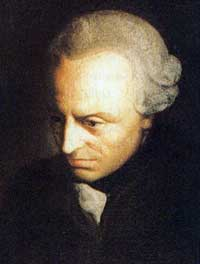
\includegraphics[height=4cm]{../../graphics/kant.jpg}
            \end{column}
            \begin{column}{7cm}
                \small{\textbf{FIRST FORMULA}}
                \begin{itemize}
                    \item \small{\alert{The Formula of Universal Law}}
                    \item \small{\alert{The Formula of the Law of Nature}}
                \end{itemize}
                \small{\textbf{SECOND FORMULA}}
                \begin{itemize}
                    \item \small{\alert{The Formula of Humanity}}
                \end{itemize}
                \small{\textbf{THIRD FORMULA}}
                \begin{itemize}
                    \item \small{\alert{The Formula of Autonomy}}
                    \item \small{\alert{The Formula of the Kingdom of Ends}}
                \end{itemize}
            \end{column}
        \end{columns}
\end{frame}

\end{document}
